\chapter{基于传统特征与深度特征融合的无线调制方式识别技术研究}
\section{引言}
在机器学习领域,经常使用融合的方法解决分类或者回归等问题,按不同层次划分,主要有数据融合、特征融合、模型融合。
特征融合主要是基于信息融合思想,通过融合不同特征对于问题的不同表征形式,
从不同层次、不同特征空间、不同时间尺度、差异性全局特征和局部特征等不同层面,对特征进行重新组合,
来提高模型的性能和鲁棒性\cite{刘渭滨2017模式分类中的特征融合方法}。\par

在上一章中,我们可以得到,CAE对调制信号所提取的特征可以重构原始信号并具有一定的类可分性;
CNN提取的特征具备较强的类可分性。
因此,我们可以利用CAE、CNN等网络,提取数据样本具备一定类可分性的深度特征。\par

在本章中,我们将CAE-CNN算法提取的卷积特征与传统特征进行融合,研究深度特征与传统特征结合对分类准确率的影响;
同时,我们也对不同的特征融合框架进行探索,研究不同的融合方式对于特征融合效果的影响。\par

\section{传统特征}
基于统计机器学习的调制识别方法,主要思想是特征提取以及模型训练;
基于D-S证据理论和判决理论的方法主要依赖特征的选择和判决门限的设定。
因此,对于传统的调制识别方法,特征的选择与提取是影响系统性能的重要条件,决定了算法所能达到的上限。
不同调制方式我们所提取的特征主要包括:时域特征、频域特征、高阶统计量等。
本章针对这几类特征集中的部分特征,利用原始数据进行提取,作为特征融合的传统特征集。\par

\subsection{基本时频特征}

我们假设原始信号$x(t)$解析表示为:
\begin{equation}
\label{eqt_4_1}
s(t)=x(t)+i*y(t)
\end{equation}
其中,$y(t)$为实信号的希尔伯特(Hilberrt)变换。\par

无线信号的调制信息主要以信号的瞬时幅度、瞬时频率和瞬时相位等特征进行表征,合理地选择和构造信号的的统计量是获得信号调制方式的重要方法\cite{杨杰2014通信信号调制识别}。\par

(1) 零中心归一化瞬时幅度谱密度的最大值\par
$\gamma_{max}$表征了信号瞬时幅度变化的统计特性,反映了无线信号的调制包络的变化情况。我们可以通过设置一定的判决门限,来区分恒定包络和非恒定包络的不同调制信号:
\begin{equation}
\label{eqt_4_2}
\gamma_{max}=max|DFT(A_{cn}(t))|^{2}/N_s
\end{equation}
其中,$N_s$为取样点数,$A_{cn}(t)=A(t)/m_a-1$为零中心归一化瞬时幅度,
$m_a=\frac{1}{N_s}\sum_{i=-1}^{N_s}A(t)$为瞬时幅度$A(t)$的平均值,
用平均值对瞬时幅度进行归一化的目的是消除信道影响。\par

(2) 零中心归一化非弱信号瞬时幅度标准差$\delta_{da}$\par
\begin{equation}
\label{eqt_4_3}
\delta_{da}=\sqrt{\frac{1}{C}\left[\sum_{A_n(i)>a_t} A_cn^2(i)\right]
	- \left|\frac{1}{C} \sum_{A_n(t)>a_t} A_cn(i)\right|}
\end{equation}
其中,$C$是全部N个采样数据中属于非弱信号值的个数,非弱信号是指幅度大于幅度判决门限电平$a_t$的信号。
$\delta_{da}$表征一个符号区间内信号的幅度变化信息,可以用来区分一个符号区间内归一化中心瞬时幅度的调制方式和归一化中心瞬时幅度不为零的调制方式。

(3) 零中心归一化瞬时幅度绝对值的标准差$\delta_{aa}$\par
\begin{equation}
\label{eqt_4_4}
\delta_{aa} = \sqrt{\frac{1}{N}\left[\sum_{i=1}^{N} A_{cn}^2(i)\right]
	- \left[\frac{1}{N} \sum_{i=1}^{N} \left|A_{cn}(i)\right|^2\right]}
\end{equation}
$\delta_{aa}$表征了信号的绝对幅度信息,可区分非归一化的绝对幅值信息和
归一化的绝对幅值信息的不同调制类别。

(4) 零中心归一化瞬时幅度的四阶紧致性$\mu_{42}^{a}$\par
\begin{equation}
\label{eqt_4_5}
\mu_{42}^{a} = E\left[A_{cn}^{4} (t) \right] / E\left[A_{cn}^{2} (t) \right]
\end{equation}
$\mu_{42}^{a}$是用来度量“瞬时幅度分布的密集性”的特征值,
可以用来区分瞬时幅度高密集分布信号和瞬时幅度分布比较分散的信号。

(5) 零中心归一化瞬时频率均值的平方与方差之比$R_f$\par
\begin{equation}
\label{eqt_4_6}
R_f = u_f^2 / d_f
\end{equation}
式\ref{eqt_4_6}中,$u_f$和$d_f$分别代表信号零中心归一化瞬时频率均值和方差。
此参数可用来判断信号是否含有频率信息。

(6) 零中心非弱信号段归一化瞬时频率绝对值的标准差$\delta_{af}$
\begin{equation}
\label{eqt_4_7}
\delta_{af} = \sqrt{\frac{1}{c}\left[\sum_{a(i)>a_i} f_N^2(i)\right]
	- \frac{1}{c}\left[\sum_{a(i)>a_i} \left|f_N(i)\right|^2\right]}
\end{equation}
其中$\delta_{af}$表征信号的绝对频率信息,可用来区分归一化中心瞬时频率绝对值为常数的调制方式和
具有绝对、直接频率信息的调制方式。

\subsection{高阶累积量}

由于码元序列的高阶统计量能够反映星座图的分布特征,适合于区分幅度相位调制方式,并具有抗噪声等优点,
因此基于高阶统计量特征的调制识别算法也是一类有效的分类算法\cite{张利2017基于高阶累积量的调制识别算法的研究}。\par

对于零均值的高斯白噪声信号,三阶及三阶以上的高阶累积量为零。
根据这一特性,求取接收信号$r(t)$的高阶累积量就是求取发送信号$s(t)$的高阶累积量。
从而高阶累积量在对零均值高斯白噪声具有有效的抑制作用以及其它一定程度上的干扰抑制。
对于不同数字调制信号的高阶累积量的值不同,而且不受零均值高斯白噪声的影响,
因此可以有效提取数字调制信号的高阶累积量为特征值,进而区分识别不同信号的调制方式。\par

对于零均值的平稳随机过程$x(t)$,其$k$阶矩定义为:\par
\begin{equation}
\label{eqt_4_8}
M_{kx} = \tau_1, \tau_2, ... \tau_{k-1} = E{x(t), x(t+\tau_1), ..., x(t+\tau_{t+\tau_{k-1}})}
\end{equation}

若考虑延时$\tau_1 = \tau_2 = ... = \tau_{k-1} = 0$,则$x(t)$的$p$阶混合矩:
\begin{equation}
\label{eqt_4_9}
M_{pq} = E\left\lbrace \left[ x(t)\right]^{p-q} 
\left[ x^*(t)\right]^{q}\right\lbrace 
\end{equation}
其中,$x^*(t)$为$x(t)$的共轭,$E{*}$为求期望。\par
根据文献[9]中的高阶矩与高阶累量的定义,我们由零均值的平稳随机过程$x(t)$的各阶累积量的公式。

(1) 二阶累积量
\begin{equation}
\label{eqt_4_10}
\begin{aligned}
C_{20} = Cum(X, X) = M_{20} = E[X(t)X(t)]\\
C_{21} = Cum(X, X^*) = M_{21} = E[X(t)X^*(t)]	
\end{aligned}
\end{equation}

(2) 四阶累积量
\begin{equation}
\label{eqt_4_11}
\begin{aligned}
C_{40}=Cum(X, X, X, X) = M_{40} - 3M_{20}\\
C_{41}=Cum(X, X, X, X^*) = M_{41} - 3M_{20}M_{21}\\
C_{42}=Cum(X, X, X^*, X^*) = M_{42} - M_{20}^2 - M_{21}^2
\end{aligned}
\end{equation}

(3) 六阶累积量
\begin{equation}
\label{eqt_4_12}
\begin{aligned}
C_{60}=Cum(X, X, X, X, X, X) = M_{60} - 15M_{40}M_{20} + 30M_{20}^3\\
C_{63}=Cum(X, X, X, X^*, X^*, X^*) = M_{63} - 9M_{42}M_{21} 
+ 9\left|M_{20}\right|^2M_{21} + 12M_{21}^3
\end{aligned}
\end{equation}

(4) 四阶累积量与二阶累积量之比
\begin{equation}
\label{eqt_4_13}
R_{mn} = |\frac{C_{42}}{C_{21}}|
\end{equation}

\section{特征融合理论}
传统的模式分类方法,主要通过特征提取,利用支持向量机、人工神经网络等算法进行分类器训练。 
但是,传统的模式分类方法通常基于人工设计的特征,经过特征提取算法得到原始数据的某些方向特征,
由于人们对于数据本身认知的片面性,很难利用特征完整的表征数据本身的分布。
这样,纯粹的基于人工特征提取训练的分类器就很难完全准确地对数据样本进行分类或者回归。\par

解决此问题的一种思路就是使用特征融合算法,利用多维特征构成的特征空间,来获取数据本身包含的性质,
弥补某些固有特征对于数据特征反映不完整的缺陷。
特征融合方法从特征层面进行处理,它既可以直接利用已有的算法提取数据特征,
相较于重新设计特征和特征提取的算法,具有较低的成本。
在本节中,我们主要研究基于深度学习的特征融合理论。\par

深度学习理论是在人工神经网络的基础上发展起来的机器学习理论,在多层神经网络中加入了更多隐层单元。
基于深度学习的特征融合算法,主要是对深度神经网络模型引入特征融合的思想,
并在模型中选择特定隐层融合其他特征,利用多源特征来训练网络参数。\par

特征融合理论主要基于两个基本假设:多特征融合通常比单特征具备更好的分类性能;融合的特征之间相关性尽量小。
前者是进行特征融合的出发点和前提,只有融合后的特征具备这样的特性,我们才具备融合的必要性。
后者是基于流形理论的假设,当特征之间的关联性较高时,融合之后的特征空间在高维流形中趋于扁平化,
可能会产生特征冗余,我们实际上可以用更小的维度来表征原始数据。
因此,我们应该从多角度选择低相关性的特征进行融合,
使数据能够在融合特征形成的高维流形中处于一个有利于我们任务(分类、回归等)的分布。\par

假设原始的数据样本集为$X$,那么对于任意${x \in X}$,
我们假设用于提取特征的隐层单元集合为$H_{hidden}$,其维度为$N$,
$h_i(x)$表示网络中第$i$个单元的输出值,则隐层神经单元构成的深度特征集为$H={h_i(x)|h_i \in H_{hidden}}$。
通过深度网络,我们可以获取原始特征空间到深度特征空间的映射:\par
\begin{equation}
	\label{eqt_4_15}
	h(x) = \bigcup_{0<i<N} w_i * h_{i}(x)
\end{equation}
当数据通过网络映射到深度特征空间的输出值,便是我们在新空间中的特征向量,即数据的深度特征。\par

同时,我们以本章中第2小节的特征提取算法,对数据的传统特征进行提取,每一个特征用$f_{i}(x)$表示,作为不同维度的特征,假设我们的传统特征集为$F$,对于任意样本$x \in X$,我们根据第2小节中的特征提取算法有:\par
\begin{equation}
	\label{eqt_4_16}
	f(x) = \bigcup_{0<i<|Z|}\mu_{i} * f_{i}(x)
\end{equation}

这样,通过融合传统特征$F$与深度特征$H$得到的融合特征集为$Z$:
\begin{equation}
\label{eqt_4_17}
	Z =F \cup H = \{ z | (z \in H) \vee (z \in F) \}
\end{equation}
最终,我们通过不同的融合算法对多源特征进行融合。特征融合的基本框架如图\ref{sec:fig_4_1}所示:

\begin{figure}[!h]
	\centering
	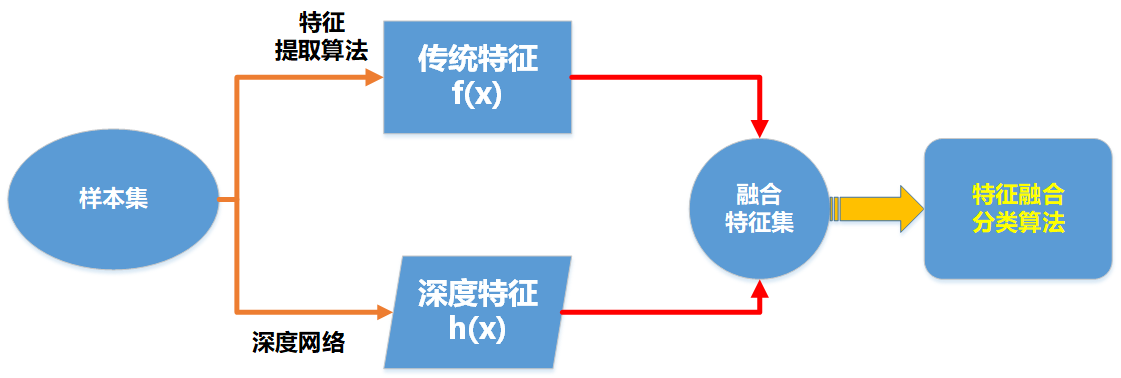
\includegraphics[scale=0.5]{figures/chapter_4/fig_4_1.png}
	\caption{特征融合框架图}\label{sec:fig_4_1}
\end{figure}

其中,XX表示我们利用的不同融合算法。在下一节中,我们将对不同融合算法的效果进行研究。


\section{传统特征与深度特征融合框架}

基于统计模式的调制识别方法也称为基于特征的调制识别方法。
这种方法把通信信号的调制
识别视为一个统计模式识别问题,整个调制识别系统由两个子系统组成:
特征提取子系统和模式分类子系统。
特征提取子系统的作用是从原始测数据中提取事先定义好的能表征信号调制类型的特征,
可以看作是从输入信号所在的观测空间到选定的特征空间的一个映射。\par

\subsection{特征归一化}
\label{sec:feature_normalization}
为了减小特征值数量级对分类性能的影响,降低梯度爆炸【】和梯度弥散对模型的影响,
我们将深度特征和传统特征进行批归一化(Batch Normalization,BN)处理。\par

假设网络的输入样本为$x$,对于特定的$mini-batch: \beta=\{x_{1,2,...,m}\}$
数据流向融合的分类器之前,对其进行归一化:
\begin{equation}
	\label{eqt:4_18}
	\hat{x_i} \leftarrow \frac{x_i - \mu_\beta}{\sqrt{\delta_\beta^2 - \epsilon}}
\end{equation}
$x_i^{(k)}$表示融合算法的第$i$个输入单元,
$\mu_\beta \leftarrow \frac{1}{m}\sum_{i=1}^{m} x_i$ 表示该单元$mini-batch$样本输入的均值,
$	\delta_\beta^2 \leftarrow \frac{1}{m}\sum_{i=1}^{m}(x_i - \mu_\beta)^2$表示该单元$mini-batch$样本输入的标准差,
$\epsilon$ 是为了防止除数为$0$而增加的偏移值,此处我们取$0.001$。\par

对于DNN融合算法,我们直接将BN作为一个完整的网络层。
由于BN本身改变了数据的分布,可能会影响到网络原有特征的表达能力了。为了恢复网络的表征能力,在对数据归一化后,又进行了还原操作$y_i \leftarrow \gamma \hat{x_i} + \beta \equiv BN_{\gamma, \beta}(x_i)$,其中$\gamma, \beta$也是通过网络的训练学习到的参数。最后,利用ADAM优化算法直接学习BN的参数和DNN的参数,获得特征与样本标记的映射关系。\par

而对于Softmax和RF融合算法,由于很难进行$\gamma, \beta$变量的学习,
所以,我们首先将数据通过网络,并获得所有样本的深度特征;
然后,基于全局的角度对包括传统特征在内的所有特征,进行如方程\eqref{eqt:4_18}所示的全局Normalization。\par

\subsection{基于Softmax回归的融合框架}

由于我们调制识别并不是一个二分类问题,
传统的$SVM$以及逻辑回归(Logistic Regression,LR)并不适应我们的应用场景。
Softmax回归(Softmax Regression, SR)模型,是LR在多分类问题上的推广。
在SR中,我们解决的是多分类问题(相应与LR解决的二分类问题),
类标$y$ 可以取 $k$个不同的值(而不是 2 个)。
因此,对于训练集 $\{ (x^{(1)}, y^{(1)}), \dots, (x^{(m)}, y^{(m)}) \}$,
我们有$y^{(i)} \in \{1, 2, \dots, k\}$。\par

对于给定的测试输入$x$,我们想用假设函数针对每一个类别j估算出概率值$p(y=j | x)$。
也就是说,我们想估计$x$的每一种分类结果出现的概率。
因此,我们的假设函数将要输出一个$k$维的向量(向量元素的和为$1$)来表示这$k$个估计的概率值。
具体地说,我们的假设函数$h_{\theta}(x)$形式如方程\eqref{eqt_4_19}:

\begin{equation}
\label{eqt_4_19}
		h_\theta(x^{(i)}) =
		\begin{bmatrix}
			p(y^{(i)} = 1 | x^{(i)}; \theta) \\
			p(y^{(i)} = 2 | x^{(i)}; \theta) \\
			\vdots \\
			p(y^{(i)} = k | x^{(i)}; \theta)
		\end{bmatrix}
			=
			\frac{1}{ \sum_{j=1}^{k}{e^{ \theta_j^T x^{(i)} }} }
			\begin{bmatrix}
			e^{ \theta_1^T x^{(i)} } \\
			e^{ \theta_2^T x^{(i)} } \\
			\vdots \\
			e^{ \theta_k^T x^{(i)} } \\
			\end{bmatrix}
\end{equation}

其中,$\theta_1, \theta_2, \ldots, \theta_k \in \Re^{n+1}$是模型的参数。
$\frac{1}{ \sum_{j=1}^{k}{e^{ \theta_j^T x^{(i)} }} }$这一项对概率分布进行归一化,使得所有概率之和为 1 。
我们有$Softmax$回归中将$x$分类为类别$j$ 的概率为:\par
\begin{equation}
p(y^{(i)} = j | x^{(i)} ; \theta) = \frac{e^{\theta_j^T x^{(i)}}}{\sum_{l=1}^k e^{ \theta_l^T x^{(i)}} }
\end{equation}

那么$softmax$回归算法的损失函数$J(\theta)$由方程\eqref{eqt_4_20}可得:
\begin{equation}
	\label{eqt_4_20}
	J(\theta) = - \frac{1}{m} \left[ \sum_{i=1}^{m} \sum_{j=1}^{k}  1\left\{y^{(i)} = j\right\} \log \frac{e^{\theta_j^T x^{(i)}}}{\sum_{l=1}^k e^{ \theta_l^T x^{(i)} }}\right]
\end{equation}
其中,$1\{\cdot\}$是示性函数,其取值规则为:$1\{ \text{True} \}=1, 1\{ \text{False }\}=0$。\par

我们通过添加一个权重衰减项$\frac{\lambda}{2} \sum_{i=1}^k \sum_{j=0}^{n} \theta_{ij}^2$来修改代价函数,这个衰减项会惩罚过大的参数值,现在我们的代价函数$J(\theta)$变为方程\eqref{eqt4_21}:\par
\begin{equation}
	\label{eqt4_21}
	J(\theta) = - \frac{1}{m} \left[ \sum_{i=1}^{m} \sum_{j=1}^{k} 1\left\{y^{(i)} 
	= j\right\} \log \frac{e^{\theta_j^T x^{(i)}}}{\sum_{l=1}^k e^{ \theta_l^T x^{(i)} }}  \right]
	+ \frac{\lambda}{2} \sum_{i=1}^k \sum_{j=0}^n \theta_{ij}^2
\end{equation}

有了这个权重衰减项以后 ($\lambda > 0$),代价函数就变成了严格的凸函数,这样就可以保证得到唯一的解了。
对$J(\theta)$的最小化问题,目前还没有闭式解法。因此,我们使用迭代的优化算法(例如梯度下降法,或 L-BFGS)。
对$J(\theta)$求导,我们得到梯度方程\eqref{eqt_4_22}。
\begin{align}
	\label{eqt_4_22}
	\nabla_{\theta_j} J(\theta) = - \frac{1}{m} \sum_{i=1}^{m}{ \left[ x^{(i)} ( 1\{ y^{(i)} = j\}  - p(y^{(i)} = j | x^{(i)}; \theta) ) \right]  } + \lambda \theta_j
\end{align}

通过最小化$J(\theta)$,我们可以得到$softmax$回归模型。
最终,基于SF的特征融合框架如图\ref{sec:fig_4_2}所示:\par
\begin{figure}[!h]
	\centering
	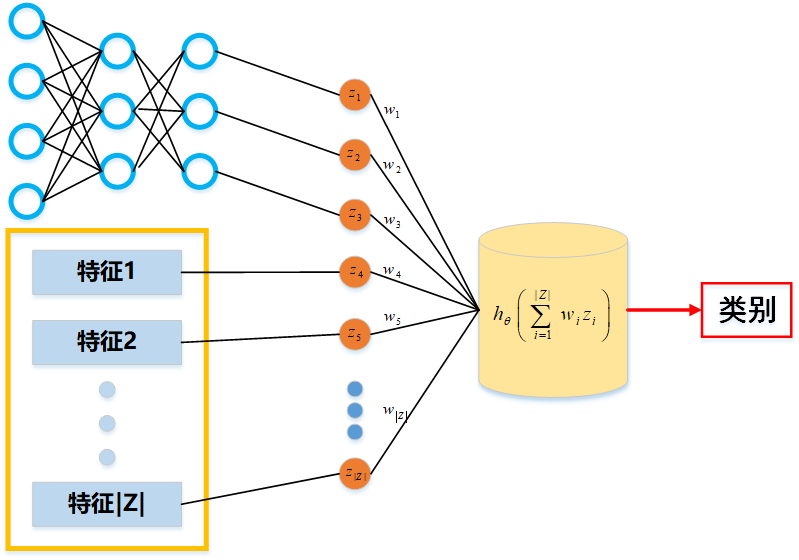
\includegraphics[scale=0.7]{figures/chapter_4/fig_4_2}
	\caption{基于LR框架的特征融合框架图}\label{sec:fig_4_2}
\end{figure}


\subsection{基于深度学习的融合框架}
随着深度学习的发展,已经有部分学者对基于深度学习的特征融合方法进行了研究。
Simonyan 等[16]首先提出了一种使用双流架构的深度卷积神经网络模型,可解决视频中的动作识别问题。
Feichtenhofer 等[15]则在这个基础上改进了网络融合方法,提出了空间特征融合方法和时间特征融合算法。\par

“如果我们的深度网络达到一定的条件,可以拟合任意的函数。“,XXX说。
DNN是对输入的数据样本,通过隐层对数据进行非线性变换,利用交叉熵或者均方误差等损失函数对隐层参数进行训练,
来输出我们希望的结果。\par

基于深度学习框架的融合方法,在融合点之前分别进行特征学习。
由本章第3小节定义,通过深度网络学习到的特征集为$H$,通过传统算法提取的特征集为$F$。\par

为降低因为特征尺度关系对后期网络学习造成的影响,我们在特征融合之前在框架中加了一个特征预处理层,
来对特征进行归一化处理。此时,我们获得的归一化特征集变为:
\begin{equation}
	\label{eqt_4_23}
	\hat{Z} =\{ f_{norm}(z) | z \in H \cup F \}
\end{equation}

融合层将独立学习的归一化特征进行融合,输入到神经网络中。
XXX等人提出了可以利用卷积层、池化层等对不同的特征进行融合处理。
我们通过对包括LSTM、DNN、CNN等框架进行验证之后,最终使用的是卷积神经网络,
并在其中加入池化层,使用dropout降低模型的过拟合风险。
在之后的深度网络层,由于样本数据有限,我们仅仅用了2层的全连接层,但是从分类结果来看,其效果还是达到预期。\par


整个基于深度学习的特征融合框架如图\ref{sec:fig_4_3}所示:
\begin{figure}[!h]
	\centering
	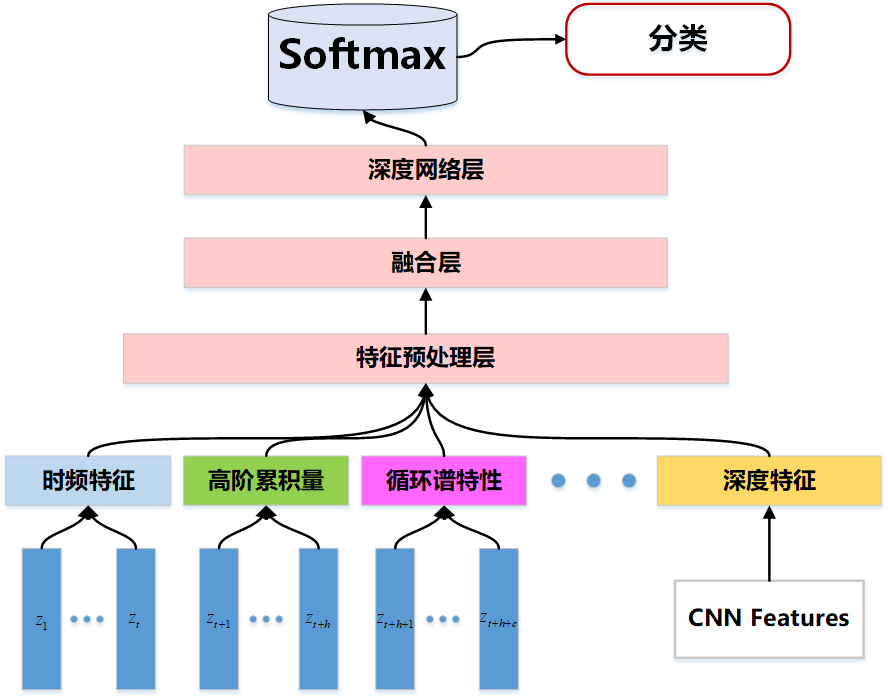
\includegraphics[scale=0.55]{figures/chapter_4/fig_4_3}
	\caption{基于DNN框架的特征融合框架图}\label{sec:fig_4_3}
\end{figure}


\subsection{基于集成树的融合框架}
集成学习通过构建并结合多个基学习器来完成学习任务,按照算法的思想它主要分为两类:Bagging族算法和Boosting族算法。\par

Bagging\cite{breiman1996bagging}是一类井行式集成学习的算法,主要基于采样数据集训练基学习器,并对这些基学习器进行组合(比如分类问题投票法、回归问题平均法)作为最终结果。Bagging主要是通过多个基学习器的集成来降低模型的方差。

Boosting算法\cite{freund1999short}的思想是先训练简单的基学习器,再根据基学习器的表现对训练样本分布进行调整,
使得先前基学习器做错的训练样本在后续受到更多关注,然后基于调整后的样本分布来训练下一个基学习器,
直至基学习器数目达到事先指定的值$T$, 最终将这$T$个基学习器进行加权结合。Boosting 主要通过过个学习器的加性组合降低偏差,其主要的代表算法是AdaBoost\cite{freund1996experiments}。\par

随机森林(Random Forest,RF) \cite{liaw2002classification}是一个基于Bagging思想的,通过随机方式建立的,包含多棵决策树的集成分类器。
它通过自助法(bootstrap)重采样技术,从原始训练样本集N中有放回地重复随机抽取k个样本生成新的训练样本集合,然后根据自助样本集生成k个分类树组成随机森林,新数据的分类结果按分类树投票多少形成的分数而定。对于我们的调制分类任务而言,随机森林简单、容易实现、计算开销小,正符合我们对集成树融合效果的验证性要求。\par


对于调制分类问题,我们将CART树(Classification And Regression Tree,CART)\cite{breiman2017classification}作为基分类器,并引入样本采样和特征采样,增加样本扰动和特征扰动对集成学习算法的影响。
基分类器的集成方法主要有平均法、投票法、stagging学习法等方法,
平均法主要是针对回归问题,而stagging的方法是利用基分类器的输出作为新的样本学习一个新的分类器,会增加模型的复杂度\cite{周志华2016机器学习}。
因此,在调制分类问题中,我们使用投票法来作为基分类器的结合方法。\par

假设我们总共学习$K$个基学习器,则每个并行训练得到的基学习器为$T_{i}$,
那么利用投票法所得的分类结果如方程\eqref{eqt_4_24}所示:
\begin{equation}
	\label{eqt_4_24}
	C(x) = \mathop{\arg\max}_{c} \sum_{i=1}^{K} I(T_i(x), c)
\end{equation}
其中,$I(T_i(x), c) \in \{0, 1\}\}$,若基分类树$T_{i}$将样本$x$预测为类别$c$,则$I(T_i(x), c)=1$,否则$I(T_i(x), c)=0$。\par

RF不仅通过样本扰动(通过对原始训练集进行采样)实现随机性,
而且通过对属性进行随机采样来增加特征的扰动,通过多棵数进行投票来预测分类结果。
这就使得最终的集成分类器的泛化性能,可通过个体学习器之间差异度的增加而进一步提升。\par
图\ref{sec:fig_4_5}展示了我们基于随机森林算法的特征融合框架图:
\begin{figure}[!h]
	\centering
	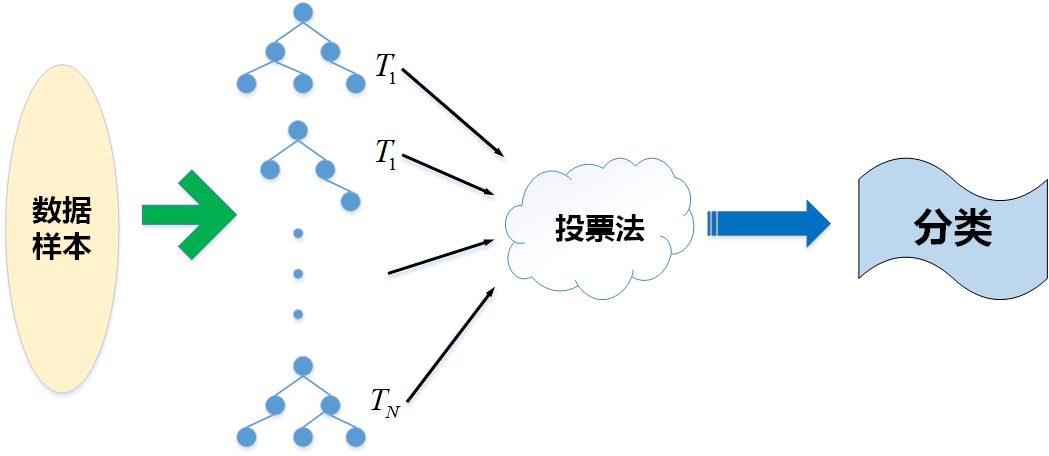
\includegraphics[scale=0.5]{figures/chapter_4/fig_4_4}
	\caption{基于随机森林框架的特征融合框架图}\label{sec:fig_4_4}
\end{figure}

\section{结果及分析}
首先,我们提取原始数据的深度特征和传统特征,并对其基于\ref{sec:feature_normalization}小节中的基准进行特征的标准化;
然后,分别基于Softmax、RF、DNN三种融合框架,学习相应的融合模型,获取特征融合之后的分类器;
最后,我们利用我们的测试数据集来对特征融合模型的性能进行验证。\par

\subsection{分类性能比较}

为了进行比较,我们将论文【】中的CNN2作为基准,与融合框架进行比较。
对于测试数据集,我们得到的不同信噪比条件下的分类准确率如图\ref{sec:fig_4_5}所示。\par

\begin{figure}[!h]
	\centering
	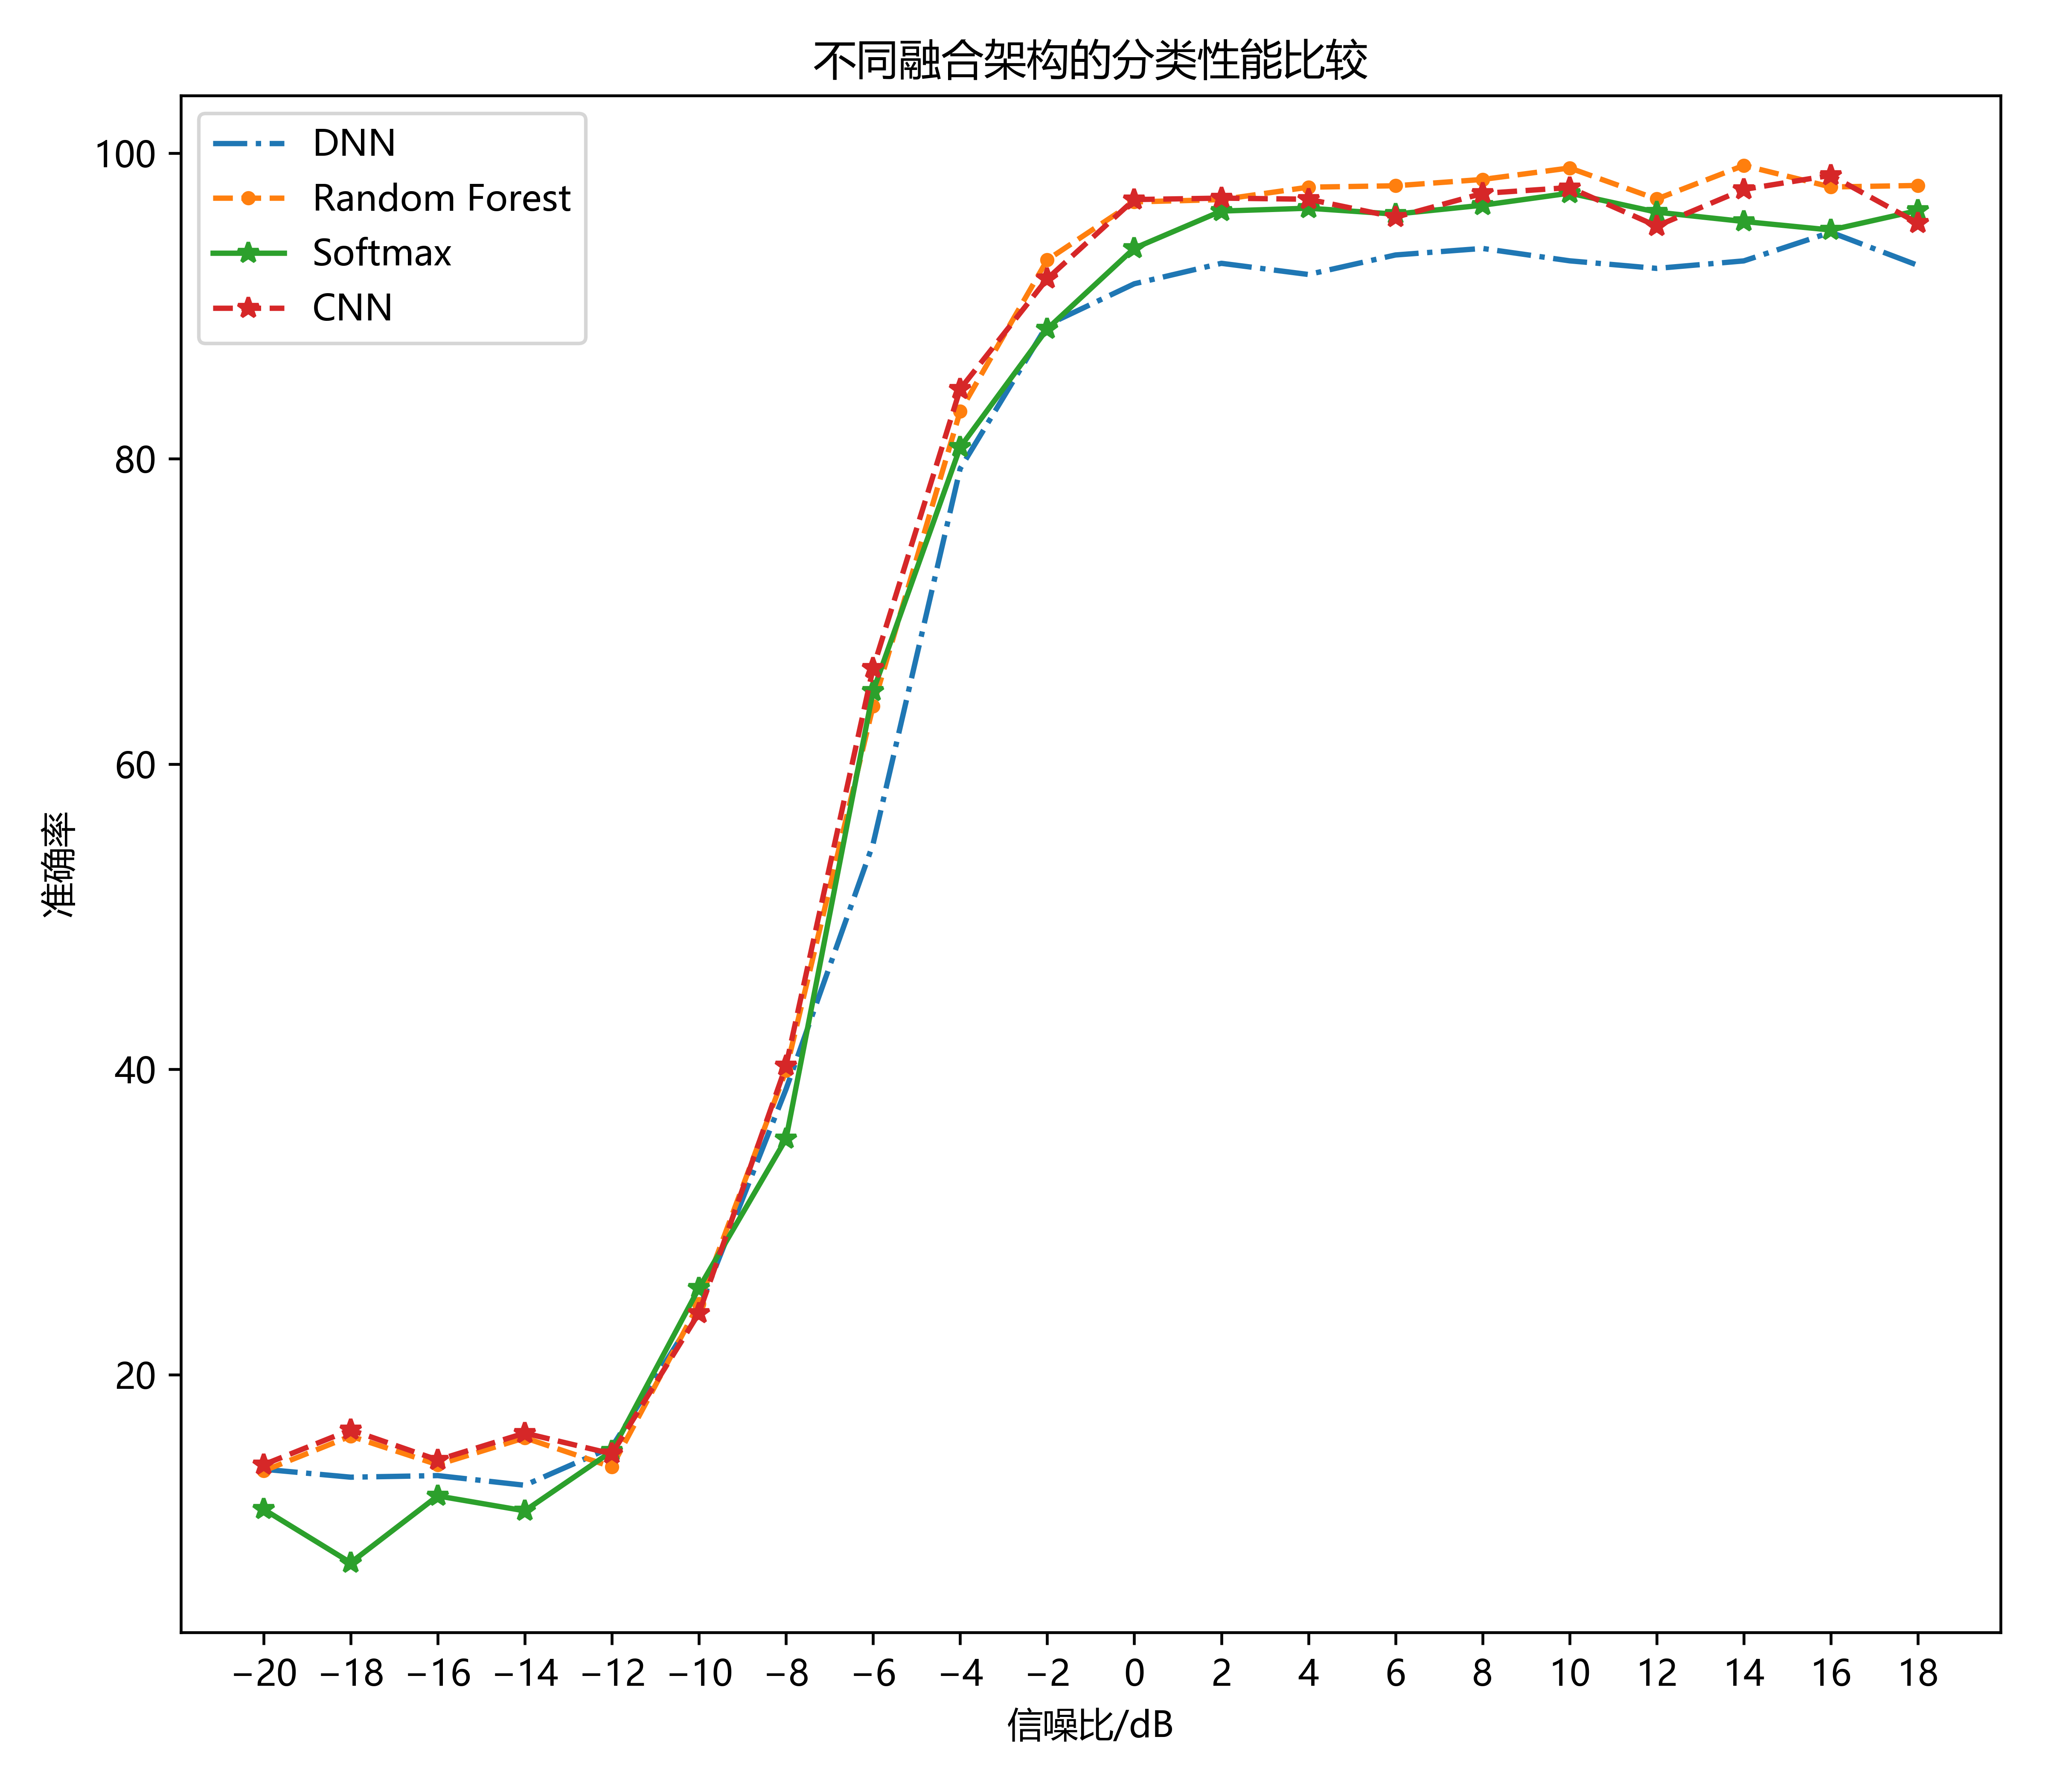
\includegraphics[scale=0.6]{figures/chapter_4/fig_4_5}
	\caption{不同融合框架下的分类性能对比}\label{sec:fig_4_5}
\end{figure}

通过图\ref{sec:fig_4_5},我们可以发现:
在高信噪比条件下,除了基于DNN融合框架的性能较差,其他三种框架的差别并不太大,
但是基于RF融合框架的模型性能更好一些,且分类性能较稳定;
在低信噪比条件下,基于RF和CNN融合框架的算法性能相近,优于其它两种算法。\par

RF本身是基于集成的思想,模型本身基于降低方差的思想,通过随机的样本采样和特征采样来降低泛化误差,对特征的波动及噪声影响泛化能力更强,因此性能可能较好。
从图\ref{sec:fig_4_5}中我们也可以发现,RF相对于其他的融合模型无论是在低信噪比还是在高信噪比性能都具有一定优势。
而对于DNN的融合模型,我们发现其性能较差,这可能是因为DNN本身拟合能力较强,而且随着网络深度增加,训练难度也会增加,泛化能力也较差,因此很难得到较好的性能。\par

\subsection{分类混淆矩阵}

我们将测试数据0dB的分类结果,构建混淆矩阵,得到结果如图\ref{sec:fig_4_6}。\par
\begin{figure}[h]
	\centering
	\subfloat[RF分类混淆矩阵]{
		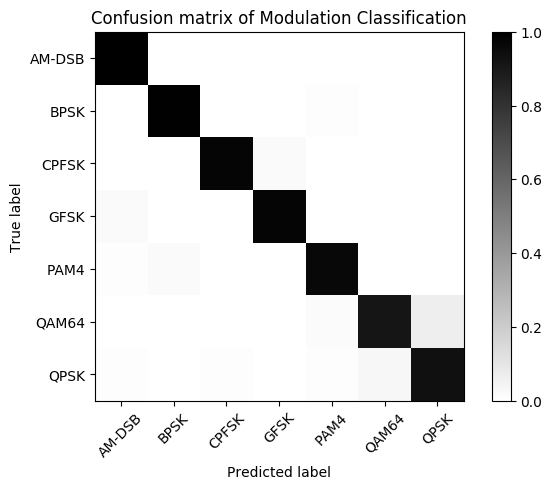
\includegraphics[width=0.5\textwidth]{figures/chapter_4/fig_4_6}
		\label{sec:fig_4_6_a}}
	\subfloat[Softmax分类混淆矩阵]{
		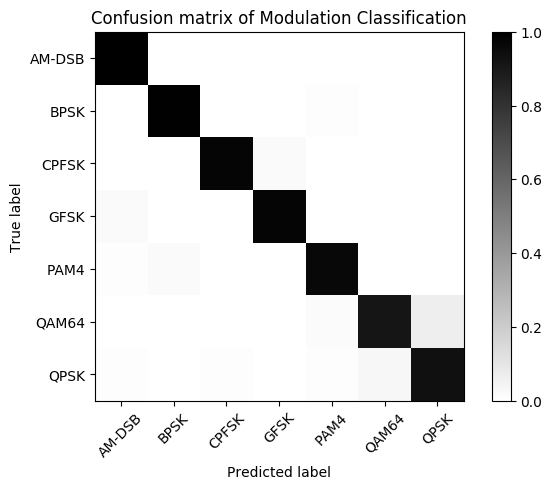
\includegraphics[width=0.5\textwidth]{figures/chapter_4/fig_4_7}
		\label{sec:fig_4_6_b}}
	\\
	\subfloat[DNN分类混淆矩阵]{
		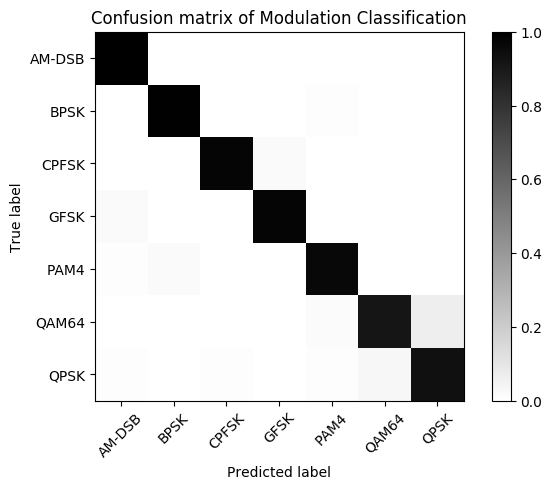
\includegraphics[width=0.5\textwidth]{figures/chapter_4/fig_4_8}
		\label{sec:fig_4_6_c}}
	\caption{不同融合模型分类混淆矩阵对比}
	\label{sec:fig_4_6}
\end{figure}

通过图\ref{sec:fig_4_6}我们可以发现三种分类器都能得到较为纯净的对角线,
但是DNN融合模型相对而言差一些,这与上一小节中的结果所得的分类结果相符,主要问题在QPSK误分为其他类别。
而基于RF和Sotfmax的模型,混淆矩阵对角线非常纯净。
基于RF的模型只有极少量的QAM样本误分为QPSK和AM-SSB,
基于Softmax的模型只有少量PAM4样本误分为AM-SSB。\par

从0dB分类结果来看,三种融合框架下的模型发生误分的信号种类并不相同,
这可能是因为模型的特性不同所致;
同时,特征标准化处理的方式不同,可能也对误分的结果产生一定的影响。
由于误差非常小,我们很难从视觉上很明显地观察出误分结果。

\section{本章小结}
基于特征层面的融合模型,能够综合利用多源特征,实现多特征的优势互补,可以获得更鲁棒、更准确的识别结果。
本章我们首先展示了融合模型中所用到的传统时频特征和高阶累积量等特征,并阐述了基本的特征融合理论,
提出了三种特征融合的算法模型,并提出了相应的算法框架下的特征标准化方法。
算法仿真结果显示,我们提出的特征融合算法中,基于RF和基于Softmax的性能优于论文【】中提出的CNN模型,
并且基于RF的融合算法具有相对最优的分类性能,无论在低信噪比还是高信噪比都具有较强的鲁棒性。
同时,受融合算法特性等的影响,不同融合框架下的误分信号各不相同。
\par
